\chapter{Compiler Architecture and Design}

In this chapter, we discuss general compiler architecture and design as well as the particular design of the reference compiler, \texttt{hyggec}.
Thereafter, we present an architecture and design proposal for \texttt{JHygge}.

From a birds eye perspective, a compiler is a program that transforms textual input data to some other representation in the form of a target language.
The target language can be many different types of languages: from low-level machine languages to other high-level programming languages.
The textual input data usually comes in the form of a data stream, either as a file stream when reading a source file or as a character stream when
reading user input from a console or tty. The most generic way to describe the typical architecture of a compiler would be the ``Pipes and Filters''
architectural pattern. In this pattern, the program consists of independent stages of data transformations, which are connected as a unified system.
As the name of the pattern suggests, there are two types of elements in this architecture: pipes and filters. Filters are stages of data transformations,
and the pipes are the connections between filters, which acts as data adapters.

The important part about the ``Pipes and Filters'' architectural pattern is that filters are completely independent of each other. One could consider
every filter to be a separate program. Thus, with the right pipe, or data adapter, any two filters could be connected. If one considers the architecture
of the \texttt{hyggec} compiler, it has a lexer/parser, a typechecker, an interpreter, an optimizer and a code generator. All of these are filters,
as they are still independent. For example, the interpreter takes an untyped AST as its input and produces an evaluation in the form of a reduced AST
and the associated side-effects. The point is that it doesn't matter how the untyped AST input is produced as this is not the responsibility of the
interpreter. Another example is the typechecker. It takes an untyped AST and produces a typed AST. It doesn't care where the untyped AST input comes
from nor where the resulting typed AST goes. This means that when viewing the \texttt{hyggec} compiler through the perspective of ``Pipes and Filters'',
any filter can be placed at any point in the pipeline, where the input and output types match. In functional programming, one could say that this is
essentially just function composition at the architectural level, as every filter can be viewed as a function with input and output types.
So this aligns well with the functional programming ideas.

\begin{figure}[H]
\centering
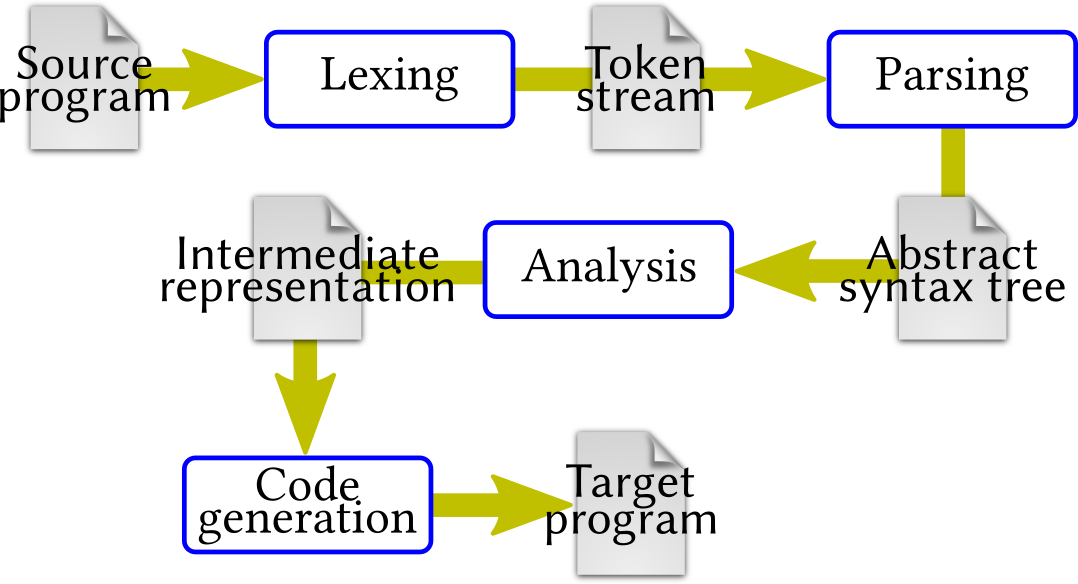
\includegraphics[width=0.3\textwidth]{Pictures/basic_compiler_phases.png}
\caption{Basic phases of a Compiler made by A. Scalas.}
\label{fig:compiler_phases}
\end{figure}

If we consider the general architecture of a compiler as illustrated by A. Scalas on figure, a compiler consists of four overall phases:
lexing, parsing, analysis and code generation. On figure, we also see the respective inputs and outputs of each phase. If one were to
look at this from the perspective of ``pipes and filters'', the input and outputs would be the pipes and the phases would be the filters.
Going a step further, a functional programmer would perhaps claim that a general compiler is a program that consists of four functions:

\begin{itemize}
  \item $Lexing : SourceProgram \rightarrow TokenStream$
  \item $Parsing : TokenStream \rightarrow AbstractSyntaxTree$
  \item $Analysis : AbstractSyntaxTree \rightarrow IntermediateRepresentation$
  \item $CodeGeneration : IntermediateRepresentation \rightarrow TargetProgram$
\end{itemize}

As such, the definition for the function \texttt{Compiler} would be:

\begin{equation*}
  Compiler : Lexing \circ Parsing \circ Analysis \circ CodeGeneration
\end{equation*}

where $\circ$ is the function composition operator. From an Object-Oriented Design perspective, one wouldn't necessarily be thinking about the structure
of a compiler in terms of function definitions, but instead be concerned with the properties of this architecture. To achieve independent phases, or filters,
is essential that the system has low coupling (minimal dependence between unrelated components) and high cohesion (related functionality is grouped together).

\section{Compilation phases in detail}

Now that we have been acquainted with the overall structure of a general compiler, we take a closer look a each of the compilation phases in greater detail.

\subsection{Lexing}

\subsection{Parsing}

\subsection{Analysis}

\subsection{Code generation}

\section{The \texttt{hyggec} architecture and design}

\section{Architecture and Design of \texttt{JHygge}}
